\chapter{Pyramid Match Score for Detection}
\label{chp5}

\section{Introduction}

Bag-of-features~\citep{bgf} schema can be considered as the watershed between traditional and modern detection methods. Instead of considering each target object as a collection of raw optical elements, i.e., pixels, the schema tries to consider each object as a set of semantic elements or so-called object parts which are usually some strong local image features. Then one visual object is said to be a target object if it possesses some certain local features of certain numbers, while does not contain other certain local features of certain numbers. While this is quite straightforward, the very precious information encoded in local features' relative positions is left over. Following some pioneering ideas~\citep{spmk,ac30}, this chapter proposes a detection method which combines spatial and visual information of local image features in a  way pursuing both efficiency and effectiveness.

The results of Chapter \ref{chp4} is promising on the two experimental datasets, however, the efficiency is not good due to the employment of Hough transform framework.
 Besides, inferring object status in a bottom-up manner fails to capture global information of each target object from the very beginning. And this is also why recently the detection results of Hough transform based methods need refinement by discriminative methods in order to be competitive. Still the way how to use spatial information of local features is very illuminate.

 Just as said in~\citep{ac27}, Hough transform based methods and sliding-window methods are the two sides of the same coin. The method proposed in this chapter calculates confidence of a target object class for each sub-window in an image. Instead of considering each object as a collection of visual patterns (appearance of local features), the method considers each object as a set of visual-spatial patterns. One object is considered as a set of points. Each point is a digital vector, with the last two dimensions the relative $x-$ and $y-$ coordinates to object center, and SIFT after principle component analysis as the remaining dimensions. The training procedure is about collecting all such visual-spatial points into a point set, which acts as a super template. During detection, each sub-image is considered as a point set, and it is matched against the super template. The confidence is then the match score.

 The key to this method is how to define a matric or match score for two point sets. Here pyramid matching procedure is employed, not only for efficiency, but also for combining visual and spatial information from local features in an effective manner. The visual-spatial space is divided from fine to coarse. Under a certain dividing parameter, points from the two matching point sets are considered as match if they fall into the same grid, and they are excluded from the respective point sets. The procedure continues till one point set is empty. Then the numbers of matched pairs under each dividing method is counted, and a weighted sum of all these numbers are considered as the match score for two point set, which will be referred to as Pyramid Match Score, or PMS for short. The weights under all dividing methods are learned during training, and also how to divide the visual-spatial space is of great importance.

Obviously, each object is considered as a whole during detection in this method.

The proposed method also has several appealing properties, which include but not limited to:
\begin{itemize}
\item {Feasibility of sequential/batch training, which will lead to easy deployment in distributed system.}
\item {Space complexity of the model is $O(1)$. Since the capacity of the point set acting as the super template is finite, and the size of the model is limited by the capacity.}
\item {Detection time complexity not related to the size of training examples.}
\end{itemize}

This chapter is organized as follows. Section \ref{rw5} reviews most related work. Section \ref{dt5} propose the training and detecting procedure. Section \ref{exp5} gives experimental results. Section \ref{conc5} concludes this chapter.

\section{Related Work}
\label{rw5}


Detection methods still mainly follow the sliding-window schema or share similar structures with Hough transforms. While the focus of the later is to infer about object status by use each online feature as query against a well-trained codebook. These methods fail to consider target objects as a whole at the beginning. The problem of sliding-window is that it often ignores positional information when also following bag of features~\citep{bgf}. In the method of~\citep{spmk}, positional information is considered in the kernel function. Here a kernel function is usually used in classifiers, which are usually support vector machines, as introduced in~\citep{kmts}. The assumption behind~\citep{spmk} is that two images are considered as similar if they possess similar object parts at similar relative positions. Despite of the good theory, its being embedded in support vector machines as kernel function limits the efficiency of this method.


The Bag-of-features~\citep{bgf} schema successfully improves detection performance, while still there are information which are left behind in images. The positional information is not fully made use of, even the method of~\citep{kmts}. While~\citep{ac3} provides a method to model the relationship between object parts, there are two many parameters to estimate in their model, which requires large amount of training data for acceptable performance.

In the method proposed in~\citep{ac222}, each object is modeled as a graph, when matching each object with another, constrains are made not only between the two objects, but also between different features of the same object. The relationship between elements of the same object is important. However, the inefficiency of this method prevents it from directly being used for object detection, while its performance on matching the same object under different views is promising.

The method in~\citep{lbt1} instead of building some parametric or non-parametric model, directly maps the labels of similar images in the training images to the current image. In this manner, the descriptive ability of model can be left alone, which in return makes the method robust. However, this kind of methods heavily rely on the manually marked labels in the training dataset, while such labels are very expensive in human power and computation.

The method in~\citep{ac3} considers both appearance model of object parts, and the relative distance changes between object parts. While giving promising results, there are too many parameters in the model, and training is troublesome when limited training images are available.

The successes of HOG~\citep{ij4} on pedestrians are also because of its ability to encode relative spatial and visual information from each divided cells. Still the flexibility is not enough, and this leads to deformable part model~\citep{ac30,dpm1}, and its enhanced versions~\citep{ac31,dpm2}, which will be referred as DPM for short, and is currently employed by most state-of-the-art methods considering  appearance information of object parts together with the relative positional information between object parts. A root template is used to detect object as a whole, and HOG feature is usually used. When an object is detected, all possible object parts are detected accordingly. Finally, the confidence is given by the confidence of the root object, the sum of confidence of the object parts, and the cost to deploy the object parts within the root object. Latent SVM is employed in the methods for optimization while using representation of complex information. Some methods motivated by DPM try to improve DPM by providing better solution searching strategies~\citep{dpm3}.  Two recent methods~\citep{spm,spltm} try to find sparse basis of object parts to reduce the number of parameters need estimating. For efficiency, the method in~\citep{408} replace the dot operator of DPM with start-of-the-art hashing method~\citep{lsh}. There also exists hierarchical extension of DPM~\citep{hdpm}, and multi-view extension of DPM~\citep{mvdpm}.

Advantages of DPM include that it only need to encode the object parts in positive training examples, and that  some of its invariants can give promising results in real time. Still DPM heavily rely of the latent SVM, which is trained in an  expectation-maximization manner, and this stops it from adopting new training examples. While nowadays, training examples often come sequentially. A very flexible model, which will evolve with training examples is preferred. These evolvements include object part number evolving, evolving of the appearance models of object parts, and evolving of the relative positions of object parts.



The pyramid match score method is most related to methods using~\citep{pmk} or~\citep{kmts} as kernel functions, methods employ Hough transforms, and also the methods proposing efficient solution space searching techniques~\citep{bab}. The method is also related to efforts trying to encode images~\citep{spen}.


\section{Pyramid Match Score}

\label{dt5}
In this section, firstly the typical procedure of pyramid matching is reviewed, and how a match score between two point sets by using pyramid matching is defined. Then based on the defined matric, how from the training examples, a super template can be learnt and how the super template can be used for object detection in a test image is proposed. In the definition of the matching score, there are parameters very important, finally in this section, how these parameters are estimated is introduced in three sub-sections.

In the content following in this chapter, all $i$s, $j$s and $k$s are local symbols.
\subsection{Pyramid Matching}



The Pyramid Matching method is designed to find the best one-one match, as shown in Figure \ref{fig:p2}, between two point sets in a heuristic manner.

Given two point sets, ${S_1} = \{ {u_1},{u_2},...,{u_m}\}, u_i \in {R^d}
$
 and ${S_2} = \{ {v_1},{v_2},...,{v_n}\}, v_i \in {R^d}$
, there exists a best one-one matching ${\pi}^*$ that minimizes the sum of $L1$
-distances between matched pairs,

\[
{\pi ^*} = \arg \mathop {\min }\limits_\pi  \sum\limits_{{u_i} \in {S_1}} {||{u_i} - {v_{\pi (i)}}|{|_1}} \ .
\]
Here $m  \le n$, and $\pi$ maps each feature $u_i$ in $S_1$ to a unique feature ${{v_{\pi (i)}}}
$ in $S_2$. There is a 2D example in Figure \ref{fig:pms1}

The best matching exists, and can be found by simple brute-force enumeration. In special cases, the Hungarian algorithm~\citep{ha} is also applicable.

\begin{figure}
\centering
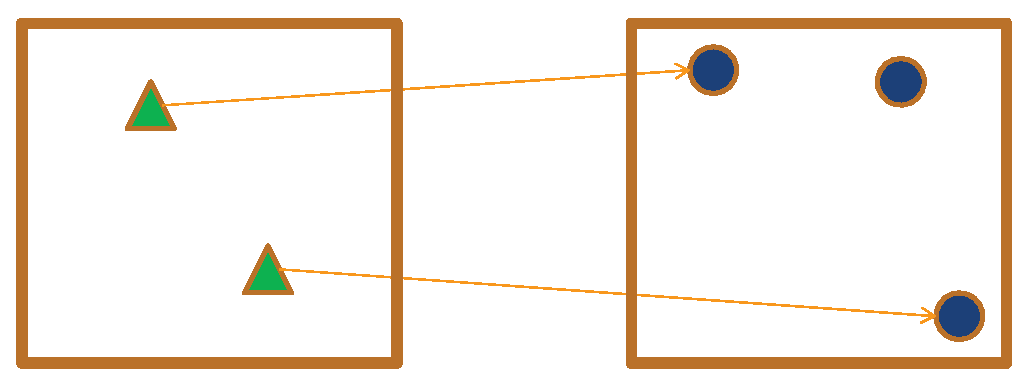
\includegraphics[width=1\textwidth]{pms1.eps}
\caption[Best one-one match.]{A best one-one match problem in 2D space. There are two points in the first point set, three in the second point set. The arrows show correspondence between the two point set.}
\label{fig:pms1}
\end{figure}

\begin{figure}
\centering
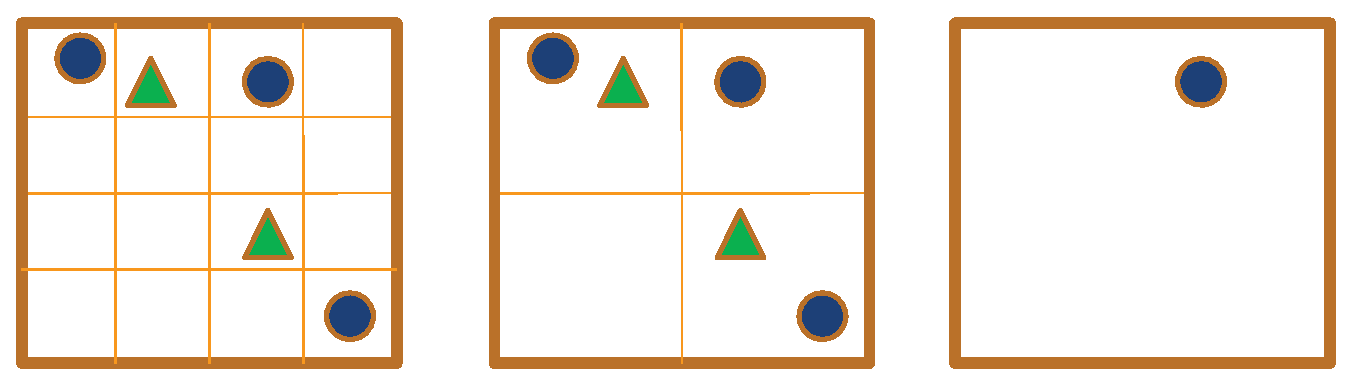
\includegraphics[width=1\textwidth]{pms2.eps}
\caption[Pyramid matching procedure.]{Pyramid matching procedure which takes the 2D one-one match problem in Figure \ref{fig:pms1} as an example. The pyramid matching method divides the 2D space from fine to coarse in the 2D space. Notice, the triangle points belong to point set one, and the circle points belong to point set two. In the left, each dimension is divided into 4, results in totally 16 grids, and no matched point pairs are found. In the middle, each dimension is divided into 2, results in totally 4 grids, and two pairs of points belonging to different point sets are found and excluded. In the right, since the matched points belonging to matched point pairs are excluded, then only one point from the second point set is left. So the number of pairs found under all dividing methods are, 0, 2, and 0. The pyramid match score is calculated as a weighted sum of these 0, 2, and 0. }
\label{fig:p2}
\end{figure}




Sub-optimal solution can be found by heuristic methods. A very intuitionistic method is to find matched pairs of nearest distance, exclude corresponding points from both point sets, and repeat until no matched pair can be found.

The Pyramid Matching method is straightforward. Divide the point space from fine to coarse, find pairs of points from different point sets in the same grid under the current dividing parameter, exclude the matched pairs, and continue this procedure until the smaller point set is empty. The Pyramid Matching method is very efficient, and its time complexity is bounded by $O(dmL)$~\citep{pmk}. Here $d$ is the number of dimensions in each point set, $m$ is size of the smaller point set, and $L$ is number of dividing methods. In the example of Figure \ref{fig:p2}, $L$ is 3.

In~\citep{pmk}, pyramid matching helps to define kernel functions for SVMs. The meaning of pyramid matching is that, it changes how the way to define similarity between two objects. Originally two objects are considered as similar if they both contain certain number of certain object parts, while the idea of one-one match will only favor the objects parts which have corresponding counterparts.

Let $\gamma  = \{ {\bf{g}_1},{\bf{g}_2},...,{\bf{g}}_L\}$ be an ordered set, which contains all the dividing methods from fine to coarse. Let $N(S_1,S_2;{\bf{g}}_i)$ be the number of matched pairs of points under dividing method ${\bf{g}}_i$. Then the pyramid match score between $S_1$ and $S_2$ on $\gamma$ is defined by,

\begin{equation}
{\rm P}(S_1,S_2;\gamma)=\frac{{\omega}_1 \times N(S_1,S_2; {\bf{g}}_1) + \sum\limits^L_{i=2}{{\omega}_i\times( N(S_1,S_2;{\bf{g}}_i)-N(S_1,S_2;{\bf{g}}_{i-1}) ) }}{m}
.
\label{eq:pms1}
\end{equation}

To exactly follow the procedure as shown in Figure \ref{fig:p2}, the definition in \ref{eq:pms1} is rewritten as,

\begin{equation}
{\rm P}(S_1,S_2;\gamma)=\frac{ \sum\limits^L_{i=1}{{\omega}_i\times N(S_1^{(i-1)},S_2^{(i-1)};{\bf{g}}_i) }}{m}
.
\label{eq:pms2}
\end{equation}

Here, $S_1^i$ and $S_2^i$ represent the point set after excluding the points which are found match after the $i$th round matching respectively from $S_1^{(i-1)}$ and $S_2^{(i-1)}$. Actually, $S_1^0=S_1$, and $S_2^0=S_2$.

The procedure is  as follow, 1) given the original $S_1$ and $S_2$, find the point pairs which fall into the same grid in the space defined by ${\bf g}_1$, 2) exclude the matched points respectively from $S_1$ and $S_2$, will lead to $S_1^1$ and $S_2^1$, and 3) continue until $i=L$ or one point set is empty.

Left behind is how to construct the dividing methods in $\gamma$ and how to define the corresponding weight ${\omega}_i$ for each ${\bf{g}}_i \in \gamma$.
And these are also the two factors which distinguish the proposed method with~\citep{pmk}.


\subsection{Training and Detection}

The Pyramid Match Score is a matric between two point sets. In~\citep{pmk}, image features are considered as points, while in the proposed method, each point encodes both appearance and location information of each local feature. Each visual-spatial point is $d-$dimensional, and, the first $(d-2)$ dimensions are SIFT after PCA, while the last 2 dimensions are relative $x-$ and $y-$ coordinates after considering scale and width-height ratio changes.

Let ${\bf{p}}$ be a visual-spatial point in the point set of an image, $I$, and  $F_{\bf{p}}$ be the image feature of ${\bf{p}}$, which is $(d-2)-$dimentional.
Let $x_{\bf{p}}$ and $y_{\bf{p}}$ be the $x-$ and $y-$ coordinates of ${\bf{p}}$.  Let $w_I$ and $h_I$ be the width and height of $I$. Then

\[
{\bf{p}}=[F_{\bf{p}}^1,F_{\bf{p}}^2,...,F_{\bf{p}}^{d-2},\frac {x_{\bf{p}}} {w_I} , \frac {y_{\bf{p}}} {h_I}]\ .
\]


Instead of following~\citep{pmk}, PMS does not server as kernel functions for SVMs. And, a procedure similar to Hough transform is employed. Each training image is considered as a point set.  From all the training images, we generate a point set as a super template, $S_{\bf{T}}$, following Algorithm \ref{alg:tm}. This is just a procedure to collect all points from point sets generated from training images into one point set.




\begin{algorithm}[chapter]





    \begin{algorithmic}[1]


       \STATE $S_{\bf{T}} \leftarrow \emptyset$

        \FOR{$S_{I_{tr}} \in \{S_{I_{tr}}\}$}

     \STATE  $S_{\bf{T}} \leftarrow S_{\bf{T}} + S_{I_{tr}}$

        \ENDFOR


    \RETURN $S_{\bf{T}}$

    \end{algorithmic}
    \caption{Template Generation}
    \label{alg:tm}


\end{algorithm}

In Algorithm \ref{alg:tm}, each $S_{I_{tr}}$ in $\{S_{I_{tr}}\}$ is the point set generated from the corresponding training image $I_{tr}$, and the $+$ operator is defined on two sets.

Actually, $S_{\bf{T}}$ plays a role similar to a codebook as in methods based on Hough transform.



For detection, a most popular pipeline is employed, as in Algorithm \ref{alg:dt}. All possible hypotheses are generated, given by $\{\eta \}$. Each hypothesis, $\eta$ is a rectangle in the image where target objects will be detected, and

\[\eta=[x_{\eta},y_{\eta},w_{\eta},h_{\eta}].\] So each $\eta$ is defined by its starting $(x,y)$ coordinate, its width, and its height. To generate $\{\eta \}$, the sliding window schema is followed, and it works by enumerating all possible rectangles by certain steps of sub-windows' positions and sizes. In Algorithm \ref{alg:dt}, ${\Omega }$ is the set of final detection results, ${\rm P}_{th}$ is a threshold to accept hypotheses as detections, $I_{te}$ is a test image, and $S_{\eta}$ is the point set generated by local features contained in ${\eta}$.


\begin{algorithm}[chapter]






    \begin{algorithmic}[1]


       \STATE ${\Omega }  \leftarrow \emptyset$, generate $\{\eta \}$ from $I_{te}$

        \FOR{$ \eta \in \{\eta \}$}

     \STATE  Calculate ${\rm P}(S_{\eta},S_{\bf{T}};\gamma)$

        \ENDFOR


    \STATE Sort $\{\eta \}$ by ${\rm P}(S_{\eta},S_{\bf{T}};\gamma)$ in descending order

    \WHILE { ${\rm P}(S_{ \eta_1},S_{\bf{T}};\gamma) >= {\rm P}_{th}$ }
     \STATE  ${\Omega }  \leftarrow  {\Omega } + \eta_1$

       \STATE  $\{ \eta \}  \leftarrow  \{ \eta \} - \eta_1$

       \FOR {$\eta \in \{\eta \}$}
       \FOR {$\eta^{'} \in {\Omega } $}
       \FOR {$\bf{p} \in S_{\eta} $}

       \IF {$({\bf{p}}^{(d-1)},{\bf{p}}^d)$ is inside $\eta^{'}$}

        \STATE  $S_{\eta} \leftarrow S_{\eta} - \bf{p} $

       \ENDIF
         \ENDFOR
       \ENDFOR
       \STATE  Calculate ${\rm P}(S_{\eta},S_{\bf{T}};\gamma)$
       \ENDFOR
        \STATE Sort $\{\eta \}$ by ${\rm P}(S_{\eta},S_{\bf{T}};\gamma)$ in descending order
    \ENDWHILE

    \RETURN ${\Omega } $


    \end{algorithmic}

    \caption{Detection Procedure}
    \label{alg:dt}

\end{algorithm}






\subsection{Dividing Visual-spatial Space}

What is very important in Algorithm \ref{alg:dt} is how to define the set of dividing methods, $\gamma$. In the method of~\citep{pmk}, ${\bf g}_i$ means dividing each dimension of the point space into $2^i$ intervals. However, the space in~\citep{pmk} is a pure feature space, while the space here is a visual-spatial space. And also, in~\citep{pmk}, the two point sets both belong to objects, while here one point set belong to the super template.

The space-dividing method proposed here divides the dimensions of visual features and spatial coordinates at different grid sizes. Let
\[{\bf g} = g(i,j),i,j \in N.\]
Here $g(i,j)$ is a function which defines how to divide the visual-spatial space. And $i$ means each dimension belonging to visual channel is divided in to $2^i$ intervals, and $j$ means each dimension belonging to spatial channel is divided into $2^j$ intervals. Note, that for a point, $\bf p$, the first $(d-2)$ dimensions belong to visual channel, while the remaining 2 dimensions belong to spatial channel. For example, if $d=3$, then $g(2,3)$ will divide the whole space into $(2^i)^{(d-2)}\times (2^j)^2=256$ grids.

In Figure \ref{fig:p3}, an example is given by considering visual information as one dimension, and spatial information the other dimension. Note, the total dimension of a point is actually $d$, while in the example it is 2.

About $\gamma$, not only its members, but also the order of its members is important. For \ref{eq:pms1} to work, a requirement must be fulfilled, that if $i<j$, ${\bf g}_i$ is finer than ${\bf g}_j$, which means if two points are decided as match under ${\bf g}_i$, they must be decided as match under ${\bf g}_j$.  This is,
 


\begin{equation}
i<j, G({\bf p}_{S_1};{\bf g}_i)=G({\bf p}_{S_2};{\bf g}_i)\mbox{     }\mbox{     }\Rightarrow \mbox{     }\mbox{     }G({\bf p}_{S_1};{\bf g}_i)=G({\bf p}_{S_2};{\bf g}_i)\ .
\label{eq:pms3}
\end{equation}

If ${\bf g}_i$ is finer than ${\bf g}_j$, it is also written as ${\bf g}_i>{\bf g}_j$.

In \ref{eq:pms3}, $G({\bf p};{\bf g})$ is a function to map {\bf p} into a particular grid, given dividing method ${\bf g}$. And $G({\bf p};{\bf g})$ on the $k$th dimension is defined by,
\[
G^k({\bf p};{g(i,j)})=
 \left\{ \begin{array}{*{20}{c}}
    \lfloor { \frac{2^i \times ({\bf p}_{max}^k - {\bf p}^k) }{{\bf p}_{max}^k - {\bf p}_{min}^k} }  \rfloor    &\mbox{  if } k \le (d-2) \\
    \lfloor { \frac{2^j \times ({\bf p}_{max}^k - {\bf p}^k) }{{\bf p}_{max}^k - {\bf p}_{min}^k} }  \rfloor  &\mbox{otherwise}
\end{array} \right. \:.
\]

Here, ${\bf p}_{max}^k$ and ${\bf p}_{min}^k$ are the maximum and minimum values on the $k$th dimension, which are determined by training dataset.



There is no such constrain which requires $\gamma$ is descending ordered by the fineness level in \ref{eq:pms2}. Thus, in the following paper, \ref{eq:pms2} will be used.
In fact, when \ref{eq:pms3} is satisfied, \ref{eq:pms1} and \ref{eq:pms2} are the same.

Though \ref{eq:pms2} can be used to calculate a pyramid match score for two point sets, given any set, $\gamma$, still the dividing methods and the order of the dividing methods will affect performance. For a largest fineness level, $l_{max},l_{max}\in N$, $\gamma$ is defined in Algorithm \ref{alg:order}.

\begin{algorithm}[chapter]





    \begin{algorithmic}[1]


       \STATE $\gamma \leftarrow \emptyset$, $r \leftarrow 2\times (l_{max}-1)$

        \WHILE {$r \ge 0$}
        \IF {$r \ge {l_{max}-1}$}
        \STATE $i \leftarrow l_{max}-1$ 
        \ELSE
        \STATE $i \leftarrow r$
        \ENDIF
        \STATE $j \leftarrow r-i$
        \WHILE {$i \le (l_{max}-1)$ \AND $i \ge 0$ \AND $j \le (l_{max}-1)$ \AND $j \ge 0$}
        \STATE $\gamma \leftarrow \gamma + g(i,j)$, $i \leftarrow i-1$, $j \leftarrow r-i$
        \ENDWHILE
        \STATE $r \leftarrow r-1$
        \ENDWHILE

        


    \RETURN $\gamma$

    \end{algorithmic}
    \caption{Set of Dividing Methods Generation}
    \label{alg:order}


\end{algorithm}



The size of $\gamma$, $L=l_{max} \times l_{max}$. For two dividing methods ${\bf g}_i,i \in {1,2,...,L}$ and ${\bf g}_j,j \in {1,2,...,L}$, if ${\bf g}_i>{\bf g}_j$, then $i<j$, which means if one dividing method is finer than the other, it will appear earlier in the set of dividing methods. There are also dividing methods, of which the fineness level cannot be compared, i.e., $g(1,2)$ and $g(2,1)$ as shown in Figure \ref{fig:p3}.


\begin{figure}
\centering
\includegraphics[width=1\textwidth]{pms3.eps}
\caption[Visual-spatial space dividing.]{An example set of methods to divide the visual-spatial space. $x-$ and $y-$ coordinates represent visual and spatial information respectively. From left to right, the first line is $g(2,2)$, $g(1,2)$, and $g(0,2)$. The second line is $g(2,1)$, $g(1,1)$, and $g(0,1)$. And the third line is $g(2,0)$, $g(1,0)$, and $g(0,0)$. And $\gamma$ is defined as an ordered set of all the dividing methods with different parameters, i.e., $\gamma=\{g(2,2),g(1,2),g(2,1),g(0,2),g(1,1),g(2,0),g(0,1),g(1,0),g(0,0)\}$.}
\label{fig:p3}
\end{figure}



\subsection{Deciding Weights for Dividing Methods}
After how to divide the visual-spatial space is decided, the remaining task is, for each dividing method $\bf g$, defining a corresponding weight.
When talking about two points which are found in the same grid under ${\bf g}=g(i,j)$, there is an upper bound to their $L1$-distance, which is given by
\[D_{ub}=  {(d-2)\times \frac 1 {2^i} +2\times \frac 1 {2^j} } ,
\]
 if unit length is assumed for all $({\bf p}_{max}^k - {\bf p}_{min}^k ),k \in \{1,2,...,d\}$. Since the first $(d-2)$ dimensions of each grid under $g(i,j)$ possess length of $\frac 1 {2^i}$, while the last 2 dimensions possess length of  $\frac 1 {2^j}$.



Following~\citep{pmk}, for two point from different point sets, if they are in the same grid under $g(i,j)$, which means $G({\bf p}_{S_1};g(i,j))=G({\bf p}_{S_2};g(i,j))$, the visual difference between ${\bf p}_{S_1}$ and ${\bf p}_{S_2}$  is defined as $ \frac {(d-2)}{2^i}$, and the spatial difference is defined as, $ \frac 2 {2^j}$.
A weight, $\omega$, defined for a dividing method $g(i,j)$ shows the importance of two matched points, and measures how difficult it is to match under such dividing method.

\begin{equation}
\label{eq:pms4}
\omega_{g(i,j)}=\sqrt{ ((d-2)\times{2^i})\times(2 \times {2^j})  }.
\end{equation}

As is seen in \ref{eq:pms4}, the finer one grid is in $g(i,j)$, the larger a weight will be assigned for it. The weight is the confidence that the point set belong to a target object based on a point has corresponding evidence from the super template under the current $\bf g$.

\subsection{Learning Weights for Dividing Methods}
Besides directly assigning weights to all the dividing methods in a deterministic way, a framework for learning weights is here proposed.

Often Gaussian kernels are used to measure differences between two features or two positions in Hough transform based methods~\citep{lb1}. 
For two visual-spatial points found match in the same grid under dividing method, $g(i,j)$,
the visual difference  is  $ \frac {(d-2)}{2^i}$, and the spatial difference is  $ \frac 2 {2^j}$.
The total difference between two points found match in the same grid is modeled using a 2D Gaussian kernel, as

\begin{equation}
\label{eq:pms5}
\omega_{g(i,j)}=\frac 1 {2 \pi \sigma_1 \sigma_2 \sqrt{1-\rho^2} }\exp(- \frac 1 {1-\rho^2} ( \frac {(\frac {(d-2)}{2^i})^2} {{\sigma_1}^2}
+ \frac {(\frac {2}{2^j})^2} {{\sigma_2}^2}  - \frac {2 \rho \frac {(d-2)}{2^i}  \frac 2 {2^j}}{\sigma_1 \sigma_2} )). 
\end{equation}

%, and here reflects the confidence the whole point set is a target object based on the current matched pair.

In \ref{eq:pms5}, $\rho$ is the correlation between visual and spatial channel, while $\sigma_1$ and $\sigma_2$ are standard deviations for visual and spatial channel.

To make \ref{eq:pms5} clear, we write it as,

\begin{equation}
\label{eq:pms6}
\omega_{g(i,j)}= t \exp(-a (\frac 1 {2^i})^2 - b (\frac 1 {2^j})^2 + c (\frac 1 {2^i}) (\frac 1 {2^j})).
\end{equation}

Where,
\[\begin{aligned}
&t= \frac 1 {2 \pi \sigma_1 \sigma_2 \sqrt{1-\rho^2} } , \\
&a= \frac {(d-2)^2  }{(1-\rho^2){\sigma_1}^2},\\
&b= \frac{2^2 }{(1-\rho^2){\sigma_2}^2 },\mbox{ and}\\
&c= \frac{2 (d-2) (2)  \rho  }{(1-\rho^2){\sigma_1}{\sigma_2} }.
\end{aligned}
\]

In \ref{eq:pms6}, the larger, the visual difference, or the larger, the spatial difference, the smaller the corresponding weight. This is decided by the 2D Gaussian kernel, and also this is consistent with Hough transform based methods.

In Algorithm \ref{alg:tm}, the weights are not needed, and the super template, $S_{\bf T}$, can be generated firstly. Then the performance of Algorithm \ref{alg:dt} will rely on the set of dividing method, $\gamma$, and each corresponding weight, $\omega$.


In \ref{eq:pms6}, to define weight for $g(i,j)$, besides $i$ and $j$, still there are four parameters, $t$, $a$, $b$, and $c$, need to be given. Here, $t$ is just a factor, it won't affect the results of Algorithm \ref{alg:dt}, which are the final detection results.

Here, $a$, $b$, and $c$ have their meanings. When $a$ is larger, visual information will play a more important role, and when $b$ is larger, spatial information will play a more important role. What is more interesting is that, there is $c$, which will be responsible for modeling correlating visual-spatial information. 

To estimate $a$, $b$, and $c$ for a particular $\gamma$, all positive training images, $\{I_p\}$, and negative training images, $\{I_n\}$, are used. For brevity, the pyramid match score against the super template, with defined $\gamma$, is rewritten according to \ref{eq:pms2},
\begin{equation}
\begin{aligned}
{\rm P}(S_{I},S_{\bf{T}};\gamma)&=\frac{ \sum\limits_{i,j}{{\omega}_{g(i,j)}\times N(S_I^{(i-1)},S_{\bf T}^{(i-1)}; g(i,j)) }}{m}\\
&=\frac{t \sum\limits_{i,j}{  \exp(-a (\frac 1 {2^i})^2 - b (\frac 1 {2^j})^2 + c (\frac 1 {2^i}) (\frac 1 {2^j}))  \times N(S_I^{(i-1)},S_{\bf T}^{(i-1)}; g(i,j)) }}{m}\\
\end{aligned}
\label{eq:pms7}
\end{equation}

In \ref{eq:pms7}, after summing up along $i$, and $j$ at given $\gamma$ and $S_{\bf T}$, it will be a function which changes according to $I$, $a$, $b$, and $c$. It is rewritten as ${\rm PMS}(I;a,b,c)$ for  brevity.

The objective function is written as the gap between pyramid match scores of positive training images and negative training images under normalizing condition as,

\[\begin{aligned}
&\arg \max\limits_{a,b,c} \dfrac{ \dfrac {\sum {\rm PMS}(I_p;a,b,c)}  {|\{ I_p \}|} - \dfrac {\sum {\rm PMS}(I_n;a,b,c)}  {|\{ I_n \}|} }
{\dfrac
{{\sum {\rm PMS}(I_p;a,b,c)}+ {\sum {\rm PMS}(I_n;a,b,c) }}
{|\{ I_p \}|+|\{ I_n \}|}
}\\
&\begin{aligned}
    s.t.:\mbox{ }& a>0;\\
    &b>0\;.
\end{aligned}
\end{aligned}
\]

After all positive and negative training examples are given, the objective function will only contain $a$, $b$, and $c$. For such a function, brute-force solutions will be feasible. 

So far, in Algorithm \ref{alg:tm}, how the template can be generated is defined,  , so Algorithm \ref{alg:dt} can be used for detection.


\section{Experimental Results}
\label{exp5}


\begin{figure}
\centering

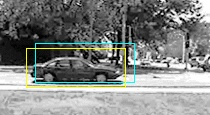
\includegraphics[scale=0.75]{test-0_good.jpg}
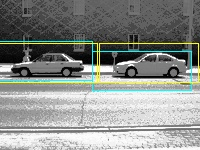
\includegraphics[scale=0.75]{test-10_good.jpg}
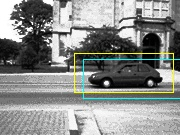
\includegraphics[scale=0.75]{test-14_good.jpg}
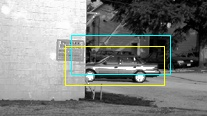
\includegraphics[scale=0.75]{test-16_good.jpg}
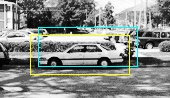
\includegraphics[scale=0.75]{test-20_good.jpg}
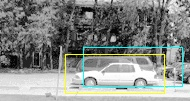
\includegraphics[scale=0.75]{test-21_good.jpg}
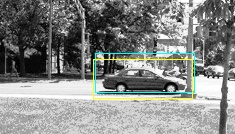
\includegraphics[scale=0.75]{test-22_good.jpg}
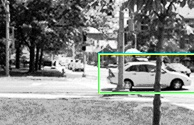
\includegraphics[scale=0.75]{test-24_good.jpg}
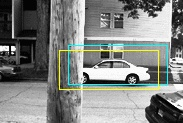
\includegraphics[scale=0.75]{test-29_good.jpg}
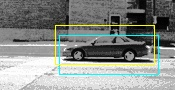
\includegraphics[scale=0.75]{test-2_good.jpg}
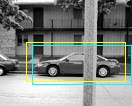
\includegraphics[scale=0.75]{test-31_good.jpg}
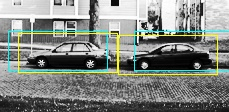
\includegraphics[scale=0.75]{test-3_good.jpg}
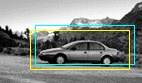
\includegraphics[scale=0.75]{test-5_good.jpg}


\caption[Detection results on UIUC cars]{Detection results on UIUC cars~\citep{cds}. Yellow color marks ground truths, while blue marks detections.}
\label{fig:c5r}
\end{figure}

In Figure \ref{fig:c5r}, are some good results on UIUC cars. And new experiments will be added.
\begin{figure}
\centering

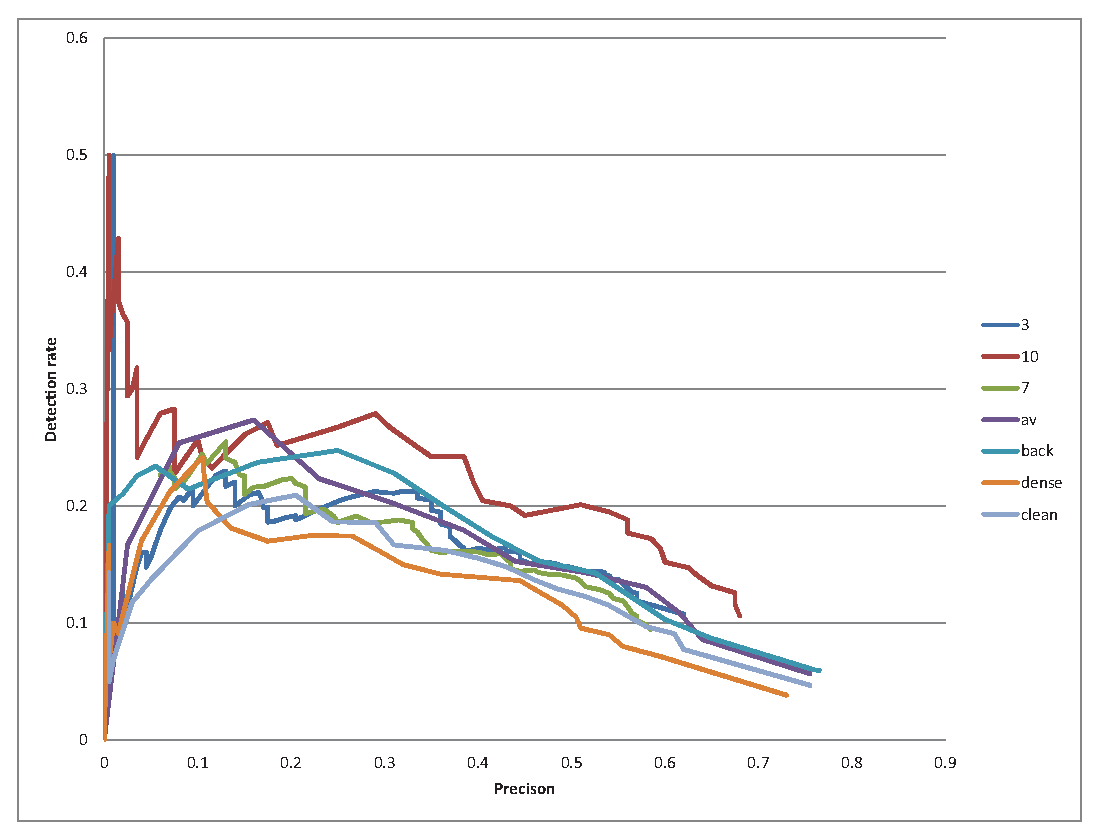
\includegraphics[width=1\textwidth]{pms.eps}


\caption[Result evaluation]{Results evaluation on UIUC cars with different implementation parameters.}
\label{fig:c52}
\end{figure}

In Figure \ref{fig:c52}, evaluations are given.

\section{Chapter Conclusion}
\label{conc5}

There will be several experiments to be summarized for this chapter, and also several experiments to be added.
